\lecture{3}{18 Sep. 14:20}{}

\section{問題的難度}


如果,
\begin{itemize}
    \item $P$ 不比 $Q$ 難且
    \item $Q$ 不比 $P$ 簡單
\end{itemize}
那兩個問題的難度相同(兩者等價)

\begin{definition}
    We say that the (worst-case) time complexity of Problem $P$ is $\Theta(f(n))$ if
    \begin{itemize}
        \item the time complexity of Problem $P$ is $O(f(n))$, i.e.
            \[
                \text{there \red{exists} an }O(f(n))\text{-time algorithm that solves Problem }P
            \]
        \item the time complexity of Problem $P$ is $\Omega(f (n))$, i.e. 
            \[
                \text{\red{any} algorithm that solves Problem }P\text{ requires }\Omega(f (n))\text{ time (in the worst case).}
            \]
        對於任何演算法,只要存在一組 instance 可以達成,一組 $\Omega(f(n))$ 即可推出
    \end{itemize}
\end{definition}

\begin{note}
若沒有特別說,$n$代表的是 input(instance) size,儲存資料所需的容量
\end{note}

\begin{note}
「正確的演算法」就是對於所有合法輸入都可以對應出正確的輸出,的解決問題方法
\end{note}

\section{演算法複雜度比較}
\[
f(n) = O(g(n)) : 
\begin{cases}
O(f(n)) = O(g(n)) \\
o(f(n)) = O(g(n)) \\
\Theta(f(n)) = O(g(n))
\end{cases}
\]

\[
f(n) = \Omega(g(n)) : 
\begin{cases}
\Omega(f(n)) = \Omega(g(n)) \\
\omega(f(n)) = \Omega(g(n)) \\
\Theta(f(n)) = \Omega(g(n))
\end{cases}
\]

\[
f(n) = \Theta(g(n)) : 
\begin{cases}
\Theta(f(n)) = \Theta(g(n))
\end{cases}
\]

\[
f(n) = o(g(n)) : 
\begin{cases}
O(f(n)) = o(g(n)) \\
o(f(n)) = o(g(n)) \\
\Theta(f(n)) = o(g(n))
\end{cases}
\]

\[
f(n) = \omega(g(n)) : 
\begin{cases}
\Omega(f(n)) = \omega(g(n)) \\
\omega(f(n)) = \omega(g(n)) \\
\Theta(f(n)) = \omega(g(n))
\end{cases}
\]

Comparing Algorithm $A$ and $B$, We say that Algorithm $A$ is \red{no worse than} Algorithm $B$ in terms of worst-case time complexity if there exists a function $f : \mathbb{N} \rightarrow \mathbb{R}$ such that
\begin{itemize}
    \item Algorithm $A$ runs in time $O(f(n))$
    \item Algorithm $B$ runs in time $\Omega(f(n))$ (\blue{in the worst case})
\end{itemize}

\begin{remark}
    第一句 Big-Oh 並沒有出現「in the worst case」是因為我們在此處分析的是「\textbf{worst case complexity}」,所以其實在 lower bound 分析的時和通常也不說。
\end{remark}

\vspace{0.7em}

Comparing Algorithm $A$ and $B$, We say that Algorithm $A$ is \red{strictly better than} Algorithm $B$ in terms of worst-case time complexity if there exists a function $f : \mathbb{N} \rightarrow \mathbb{R}$ such that
\begin{itemize}
    \item Algorithm $A$ runs in time $O(f(n))$
    \item Algorithm $B$ runs in time $\omega(f(n))$ (\blue{in the worst case})
\end{itemize}
or
\begin{itemize}
    \item Algorithm $A$ runs in time $o(f(n))$
    \item Algorithm $B$ runs in time $\Omega(f(n))$ (\blue{in the worst case})
\end{itemize}

\section{分析演算法複雜度下界}

儘管有些 case 可以,但 Big-Omega 不可以跟 Big-Oh 一樣分析(多增加)

\begin{remark}
    \redbox{\textbf{$\Omega$-time 必須要一組一組 instance 分析}}
\end{remark}

\section{問題上下界 vs 演算法上下界}
\begin{itemize}
    \item 一個問題 $P$ 的任何正確演算法 $A$ 的複雜度上界都是問題 $O(f(n))$ 都是問題 $P$ 的複雜度上界
    \item 一個問題 $P$ 的複雜度下界 $\Omega(f(n))$ 都是 $P$ 的任何正確演算法 $A$ 的複雜度下界
\end{itemize}


\chapter{演算法的設計與分析}

\section{Half Sorted}
\begin{definition}[Half Sorting Problem]
    An $n$-element array $A$ is half-sorted if
    \[
        A[i] \leq A\left[ \left\lfloor \frac{i}{2} \right\rfloor \right]
    \]
    holds for each index $i$ with $2 \leq i \leq n$.
\end{definition}

\textbf{Half-sorting Problem}:
\begin{itemize}
    \item Input: \[
        \text{An array A of n distinct numbers.}
    \]
    \item Output: \[
        \text{A half-sorted array that is reordered from A.}
    \]
\end{itemize}
\begin{note}
    正確的輸出未必唯一,因此輸入輸出就不是一個函數,而是一個 「relation」
\end{note}

\subsection{排序法 Sorting method}

\begin{theorem}
歸約 Reduction(問題重整),把問題的難度如果問題 $P$ 可以「多項式時間歸約」成問題 $Q$,就寫作

\[
    P \leq_p Q
\]

意思是:只要能解決問題 $Q$,就能透過快速轉換來解決問題 $P$,所以:
\begin{itemize}
    \item 如果 $Q$ 是容易的(有快速演算法),那麼 $P$ 也會是容易的。
    \item 如果 $P$ 已知很難,那麼 $Q$ 至少也不會比較容易。
\end{itemize}
\end{theorem}

\begin{note}
把問題的性質變強,便可以順便證明性質較弱的問題
\end{note}

\newpage


因此,我們知道用排序法一定可以解決半排法,我們可以把半排問題「歸約」到「排序」問題,因此我們首先分析一下快速排序法:


\begin{lstlisting}[language=iPython, caption=Quicksort in Python, xleftmargin=0.05\textwidth]
def qsort(A, l, r):
    if l >= r:
        return
    (i, j, k) = (l, r, A[l])

    while i != j:
        while A[j] > k and i < j:
            j -= 1
        while A[i] <= k and i < j:
            i += 1
        if i < j:
            (A[i], A[j]) = (A[j], A[i])

    (A[l], A[i]) = (A[i], k)

    qsort(A, l, i-1)
    qsort(A, i+1, r)
\end{lstlisting}

我們必須分析他的正確性及複雜度

\begin{theorem}
    The function \texttt{qsort()} is correct.
\end{theorem}
\begin{proof}
    First, we know that every round of \texttt{qsort()} will let the array become:
    \[
    A[l\ ..\ p-1] < A[p] < A[p+1\ .. \ r] \quad A[p] = \text{pivot}
    \]
    \red{(How to proof)}

    Let $m$ be the number of elements in the array. By the induction, we can start with
    \begin{itemize}
        \item Case $m=1$: The array is well sorted.
        \item Case $\forall t \leq m \rightarrow (m+1)$: Every round of iteration we can get a $p$ such that \[
            \forall x \in A[l \ .. \ p-1],\ x \leq A[p], \quad \forall y \in A[p+1 \ .. \ r],\ y \geq A[p]
        \]
        We assume that array with length equal to $t$, $\forall t \leq m$, has been sorted. Then we can know that that \texttt{qsort(A, l, p-1)}, \texttt{qsort(A, p+1, r)} is well sorted. Thus, we can combined $A[l \ .. \ p-1]$, $A[p]$, $A[p+1 \ .. \ r]$ to get a well-sorted array $A[l \ .. \ r]$ with length $m$.
    \end{itemize}
    Hence, by induction, \texttt{qsort()} is correct.
\end{proof}

\vspace{0.5em}

Then, we can stat to analyze the time complexity (worst case):



\newpage

\subsection{順調法}

\begin{definition}[順調法]
    
\end{definition}

為了方便觀察我們可以將這個陣列化成樹的形式(不是真的改變資料結構)
\begin{itemize}
    \item Each $A[i]$-to-root path is increasing
\end{itemize}

\begin{figure}[h]
    \centering
    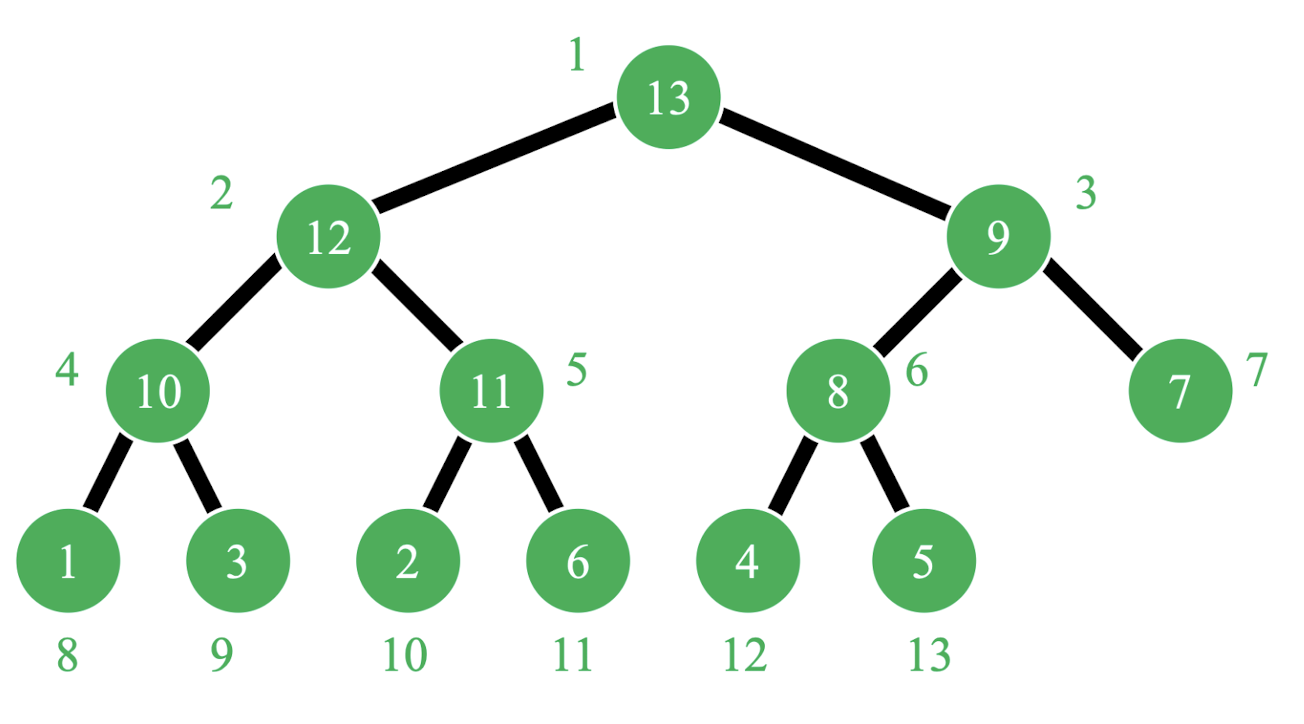
\includegraphics[width=0.55 \linewidth]{Figures/tree.png}
    \caption{Display with Tree structure}
\end{figure}

\subsection{逆調法}

\newpage
\redbox{算上面算比較少,樹的上下是不對稱的}
\newpage